\documentclass[letterpaper]{article}

\usepackage[T1]{fontenc}
\usepackage{microtype}
\usepackage{libertine}

\catcode`\_=12

\usepackage{glossaries}
\usepackage{siunitx}
\usepackage{authblk}

\usepackage{booktabs}

\usepackage{graphicx}
\usepackage{caption}
\usepackage{subcaption}

\captionsetup{font={small},labelfont=bf}

% last
\usepackage[colorlinks=true]{hyperref}

\title{Prediction of CDI Words \& Sentences values from Words \& Gestures}

\author{Trevor K.\,M. Day}
%\author[1,2]{Trevor K.\,M. Day\thanks{\url{day00096@umn.edu}}}
%\affil[1]{Institute of Child Development, University of Minnesota}
%\affil[2]{Masonic Institute of the Developing Brain, University of Minnesota}

\newacronym{cdi}{CDI}{Communicative Development Inventory}
\newacronym{ws}{WS}{Words \& Sentences}
\newacronym{wg}{WG}{Words \& Gestures}
\newacronym{icc}{ICC}{intraclass correlation coefficient}
\newacronym{rpd}{RPD}{relative percent difference}

\newcommand{\sounds}{\textit{Sound Effects and Animal Sounds}}
\newcommand{\cwords}{\textit{Connecting Words}}
\newcommand{\hverbs}{\textit{Helping Verbs}}
\newcommand{\food}{\textit{Food and Drinks}}
\newcommand{\qwords}{\textit{Question Words}}

\newcommand{\wshat}{$\hat{\textrm{WS}}$}

\begin{document}

    \maketitle

    \section{Introduction}

    The Baby Connectome Project (BCP) % CITE
    collected MacArthur-Bates \glspl{cdi} % CITE
    beyond the typical normed range of
    8--18 months. This means it is unclear how to interpret scores beyond this
    range.

    \section{Methods}

    I acquired CDI \gls{ws} data from Wordbank % CITE
    (Feb. 15. 2023), comprising $n=7905$ unique individuals with an age field
    between 16--30 months.
    The Wordbank data were divided into a training set (75\% of the data at each
    age) and a testing set (the remaining 25\%).

    All \gls{wg} items appear on \gls{ws}, with the exception of ``in'' and
    ``inside,'' which is two items on the \gls{wg} form and one on \gls{ws}. For
    the \gls{wg} score, an endorsement of the ``inside/in'' item was scored as
    two \textit{words produced}.



    Within each category, I regressed the difference against age (in months
    since 18 months, the youngest age that \gls{ws} is normed for) and the
    calculated \gls{wg} score, and the interaction between them.

        For each participant's inventory score (e.g. \sounds{}, \textit{Animals},
    $\ldots$), I calculated the total number
    of items endorsed, and the total number of items endorsed, counting only those that also
    appear on the \gls{wg} form, see \autoref{fig:allWGWS}.
    The lowest $R^2$ of the quadratic regression of \gls{ws} on \gls{wg}
    was \hverbs{} at 0.694, but the rest exceeded 0.890.

    \begin{figure}
    	\centering
    	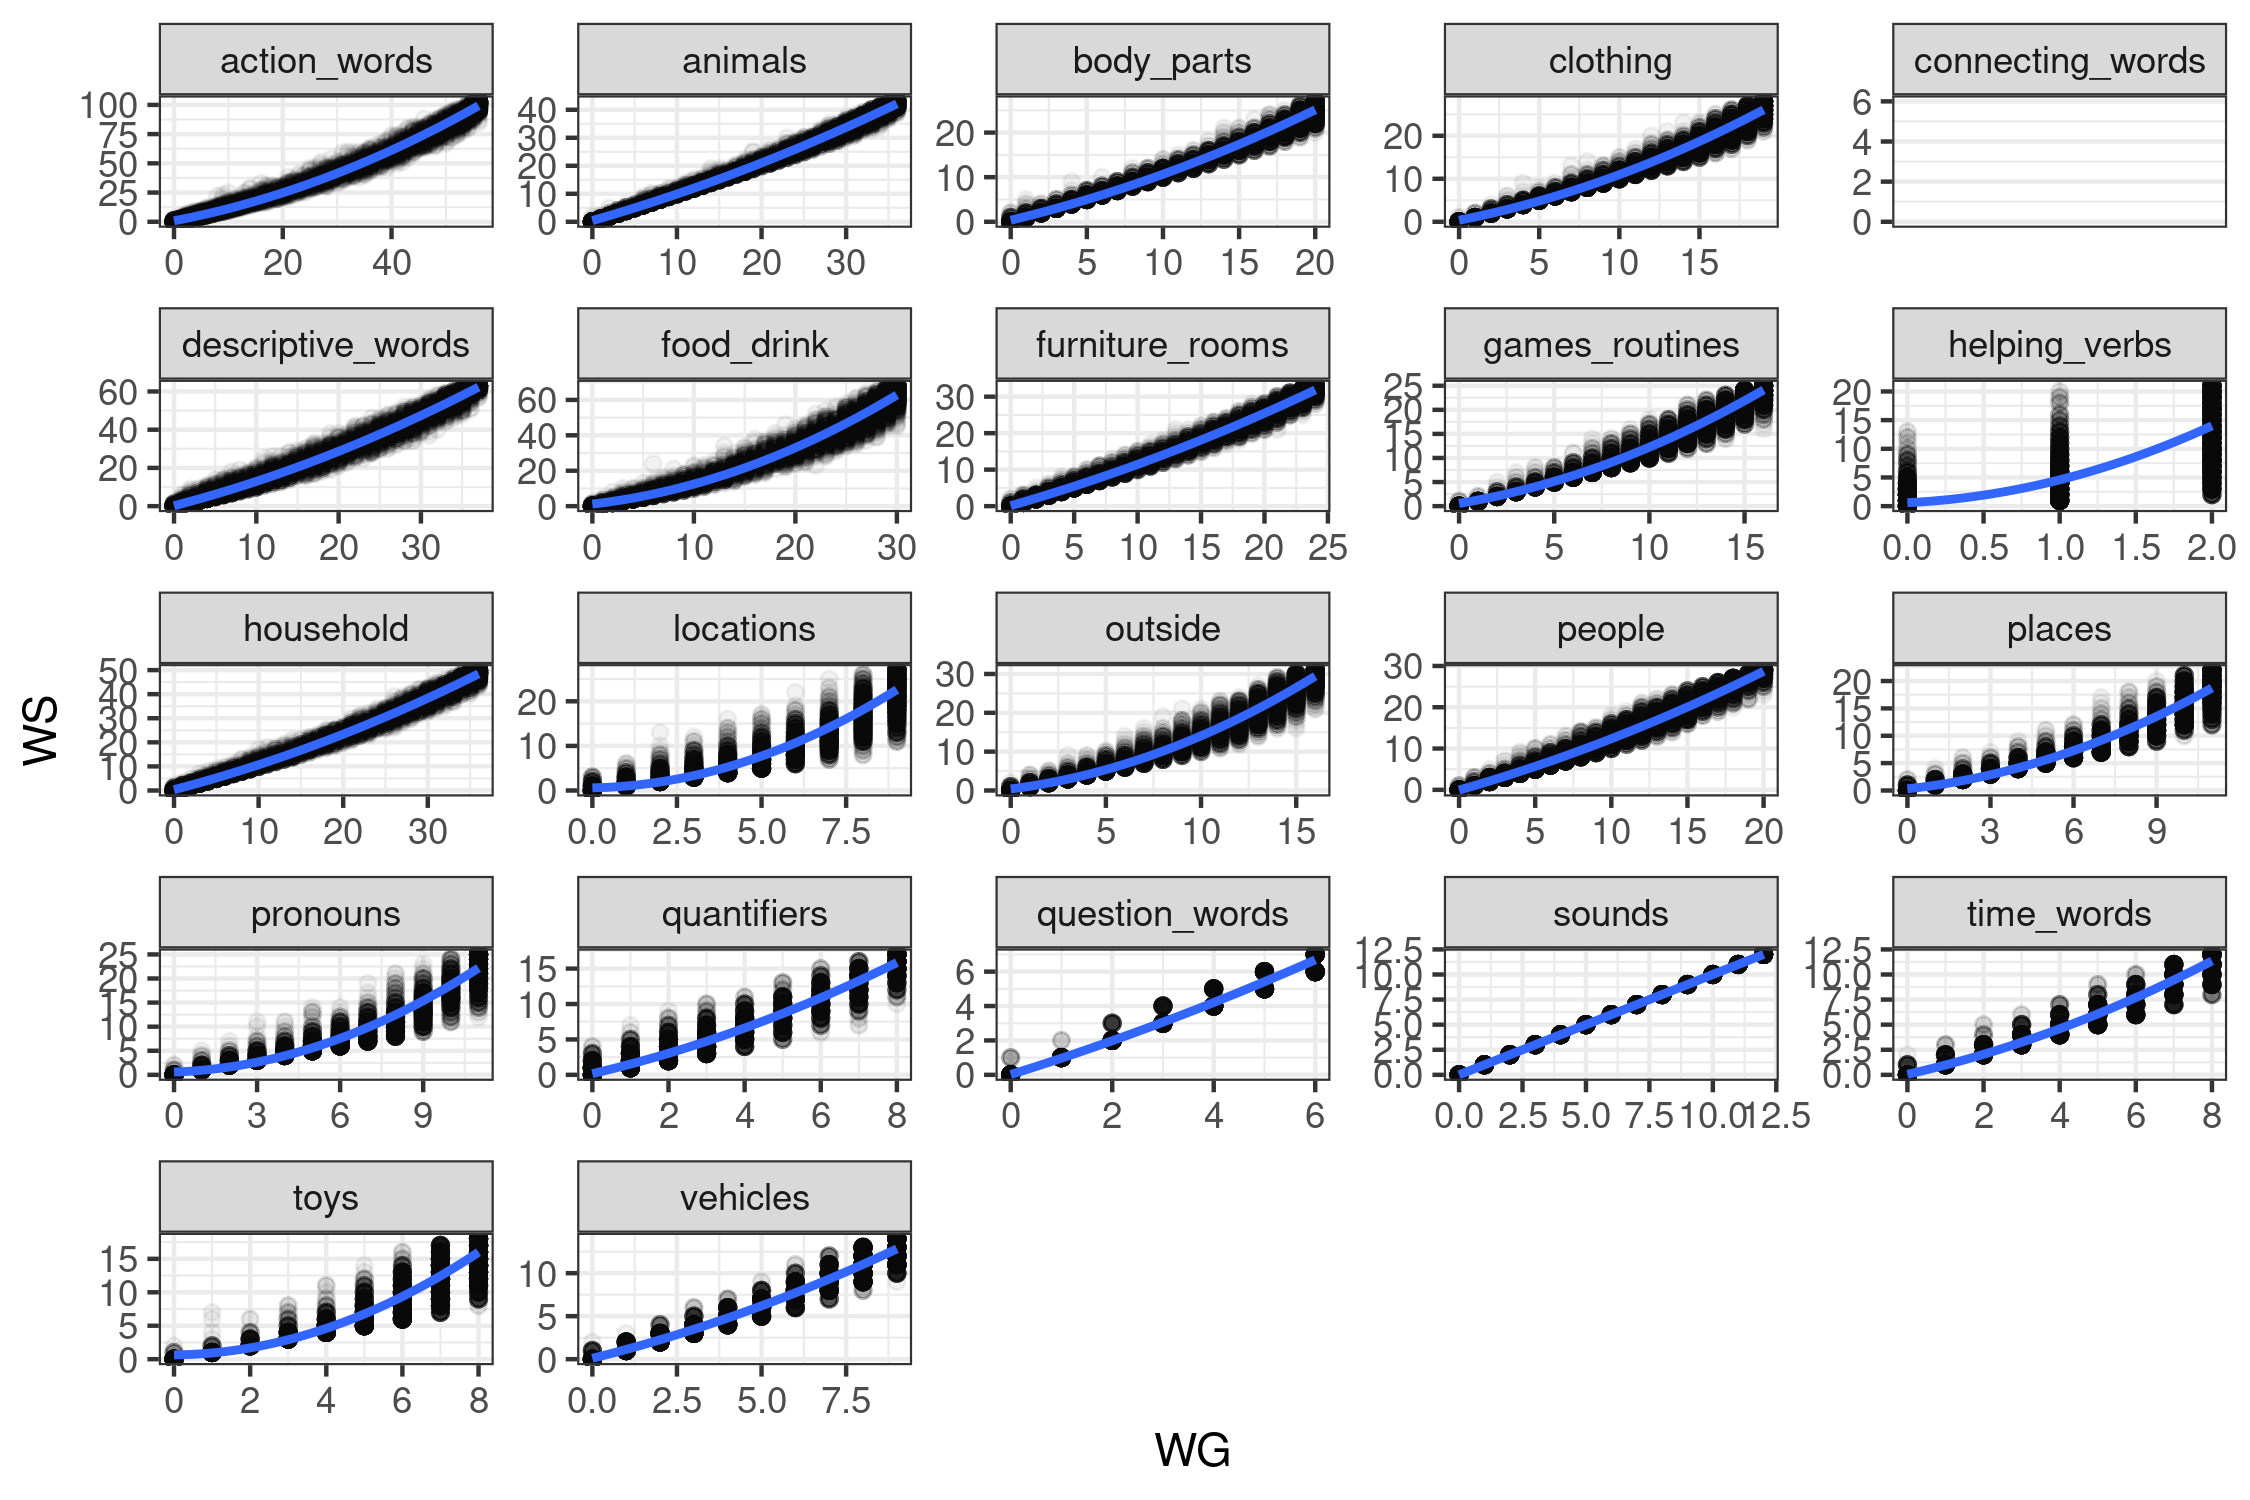
\includegraphics[width=\textwidth]{../WG2WS_plots/all_WSagainstWG}

    	% Check these for latest training/test split

    	\caption{True WS scores ($y$) against score using only WG items ($x$).
    		$R^2$ values: action words: 0.993; animals: 0.996; body parts: 0.985;
    		clothing: 0.980; connecting words: N/A;
    		descriptive words: 0.989; food/drink: 0.973;
    		furniture/rooms: 0.992; games/routines: 0.966; helping/verbs: 0.694;
    		household: 0.993; locations: 0.911; outside: 0.973; people: 0.974;
    		places: 0.942; pronouns: 0.947; quantifiers: 0.951;
    		question words: 0.99; sounds: 1.00; time words: 0.976; toys: 0.899;
    		vehicles: 0.966.}

    	\label{fig:allWGWS}

    \end{figure}

    An additional key problem is that no \cwords{} items appear on the \gls{wg}
    form. Secondly, \sounds{} is identical between the two forms. These two categories are
    ignored for the total-score analyses to be more conservative in estimates of error rate.

    \section{Results}

    The Pearson correlation between the true \gls{ws} score and the calculated
    \gls{wg} score for each individual/category was $r=0.962$ (Spearman $r=0.970$).
    Mean differences
    by category across ages are shown in \autoref{fig:diffs_by_cat}. Notably
    large differences emerge in \food{}, \textit{Action Words},
    and \textit{Descriptive Words}, whereas statistically no differences emerge
    in \qwords{}.

    \subsection{Categories}

    Within each
    category, in addition to the quadratic WG model,
    I regressed the ground-truth \gls{ws} score on age,
    \gls{wg} score, the
    age--score interaction, as well as age$^2$, WG$^2$ and the interaction of
    the quadratic terms. The quadratic terms were included because of the
    clear nonlinearity of the age effect in development, as well as the
    nonlinear effect of \gls{wg} score on true \gls{ws} score
    (\autoref{fig:allWGWS}).

    Inspection of the residuals from the second-level model suggested a nonlinear effect
    of total score, so the third-level model included the cubic effect of total \gls{wg}
    score. This offered a major cross-category improvement in AICc.

    \begin{figure}
	    \centering
	    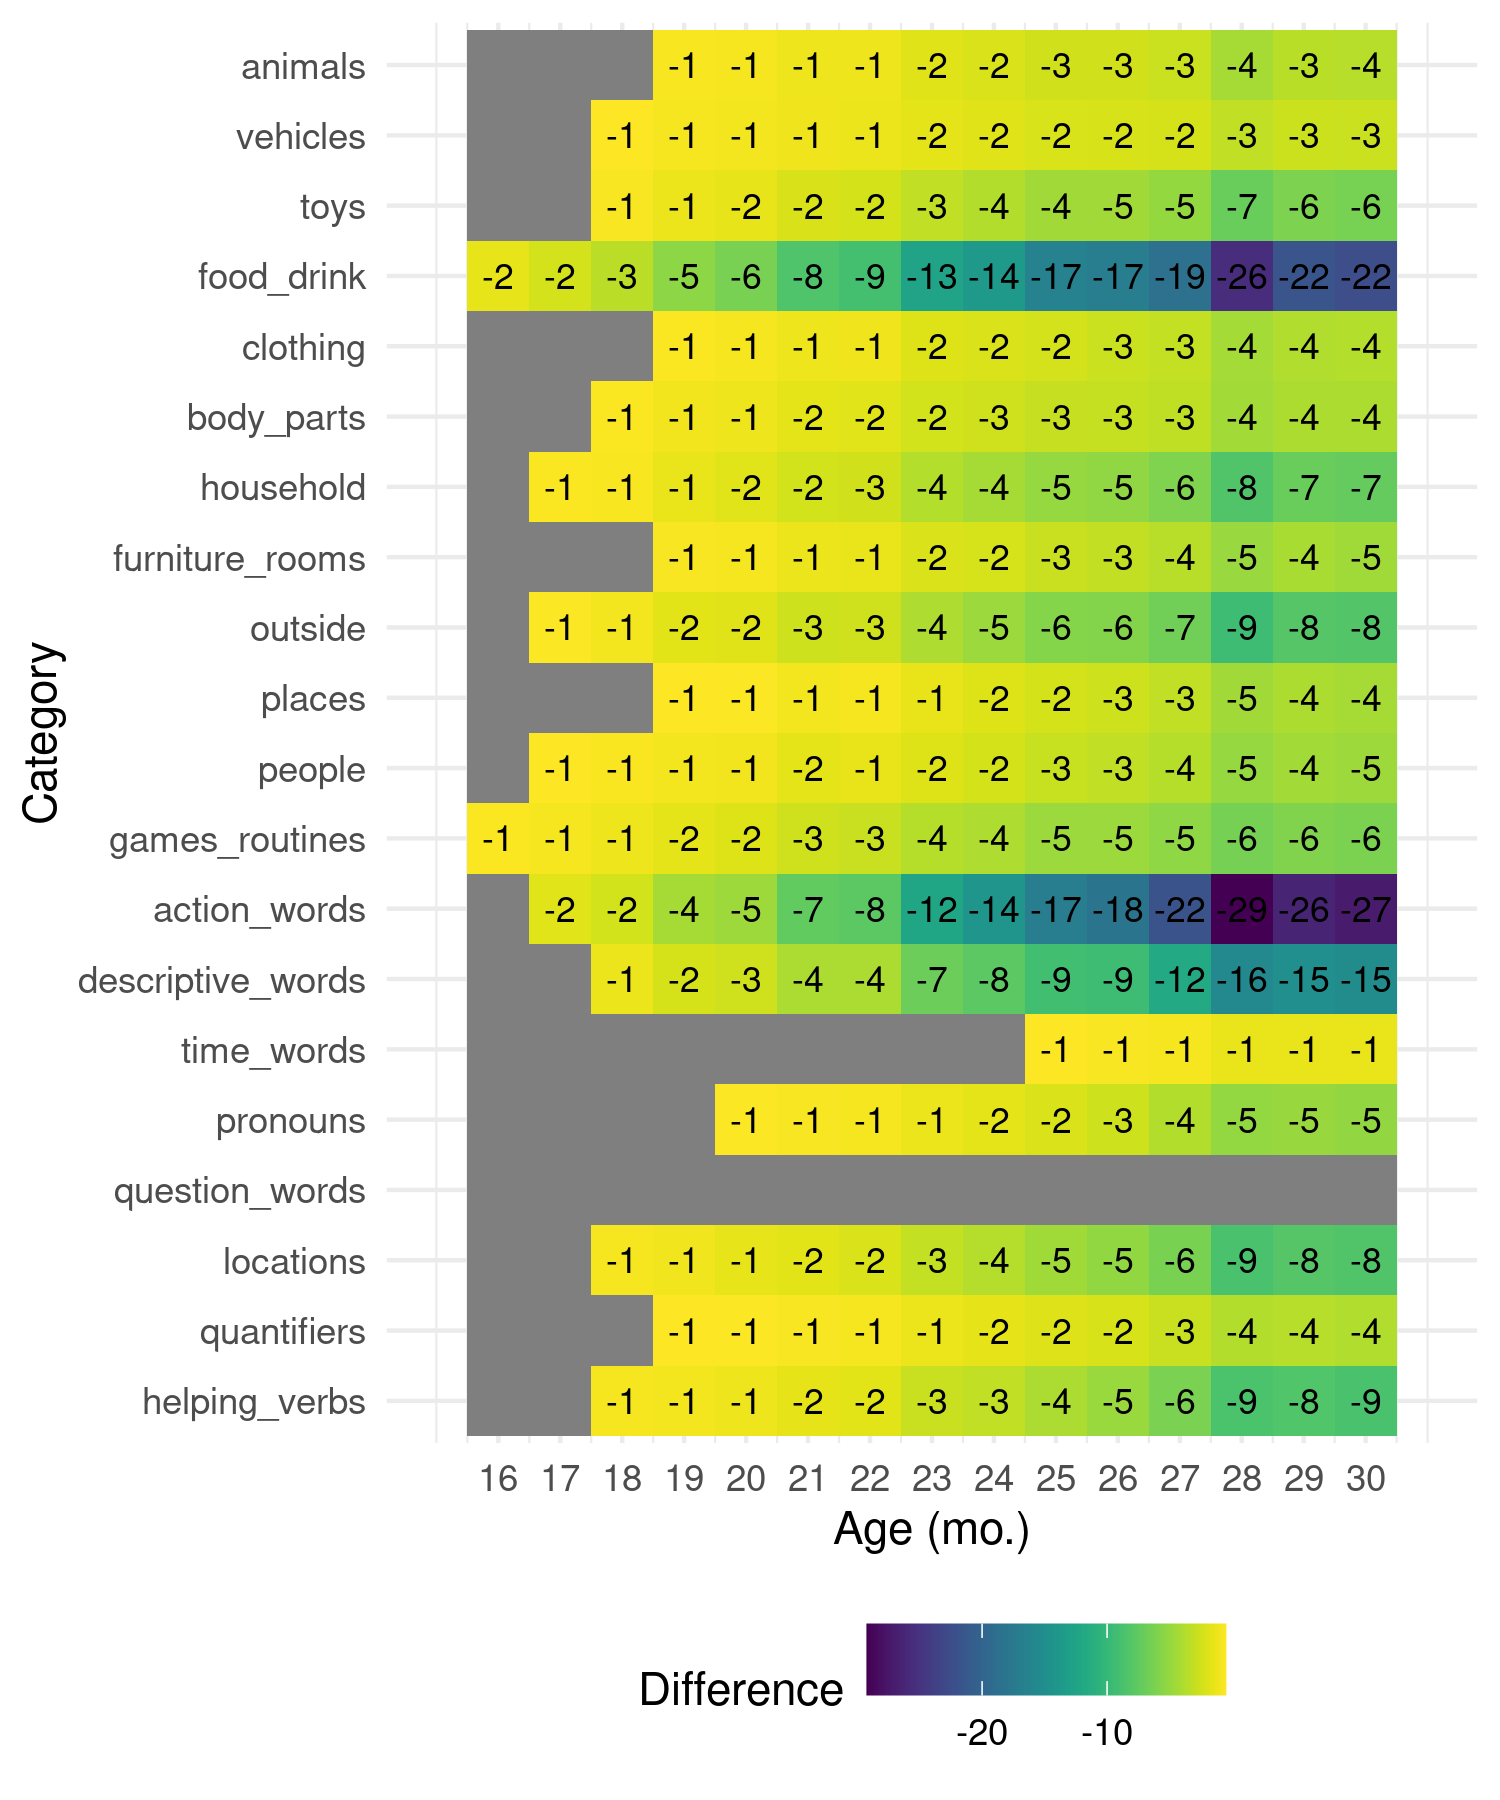
\includegraphics[width=\textwidth]{../WG2WS_plots/WGWS_diff}
	    \caption{Mean difference between score-only \wshat{} and true WS score.
	    			Non-significant differences and differences less than 1 word are
	    			omitted (gray).}
	   	\label{fig:diffs_by_cat}
    \end{figure}

	On an category level, the mean error in words was no larger than 2.36
	(\food{}). Likewise, the largest 2$\sigma$ range for the category level estimate
	was 6.55 (also \food{}), i.e. 95\% of the population was estimate correctly
	to within $\pm3.27$ words.

    \subsection{Total Score}

    The \wshat{} scores were summed to create a total predicted score (still
    excluding \sounds{} and \cwords{}). Three plots show the residuals against the
    ground truth WS score and the calculated sum WG score.

    \autoref{subfig:err} shows that 95\% of predicted scores land within $\pm23.5$ words
    (solid line, dashed line; $1\sigma=11.7$),
    with still some nonlinearity at the highest scores (ceiling effects).

    The second two plots have been log-transformed due to some extremely high
    error percentages.
    \autoref{subfig:errpct} shows the absolute error ($+0.1$, hence the line at
    $y=0.1$).
    There is a huge spike of inaccuracy at total word counts less than 50
    words. When
    individuals with fewer than 50 word are excluded, 95\% of the population is
    within 9.3\%
    of their true score.

    Finally, \autoref{subfig:errpctage} removes those with inventory scores
    less than 50 words. Furthermore, it shows there is no dependency on age;
    thus no age criterion (the blue line shows the age at which \gls{ws} is
    no longer normed.) All the participants with absolute percent error greater
    than 16\% had inventory scores between 50 and 100; suggesting that 100
    words is a more conservative lower bound for WG$\rightarrow$WS conversion;
    however, this runs the risk of eliminating data: 100 words is more than the
    50th percentile of scores in the training set until 21 months.


    \begin{figure}

        \centering

    	\subcaptionbox{Error in words\label{subfig:err}}
    		{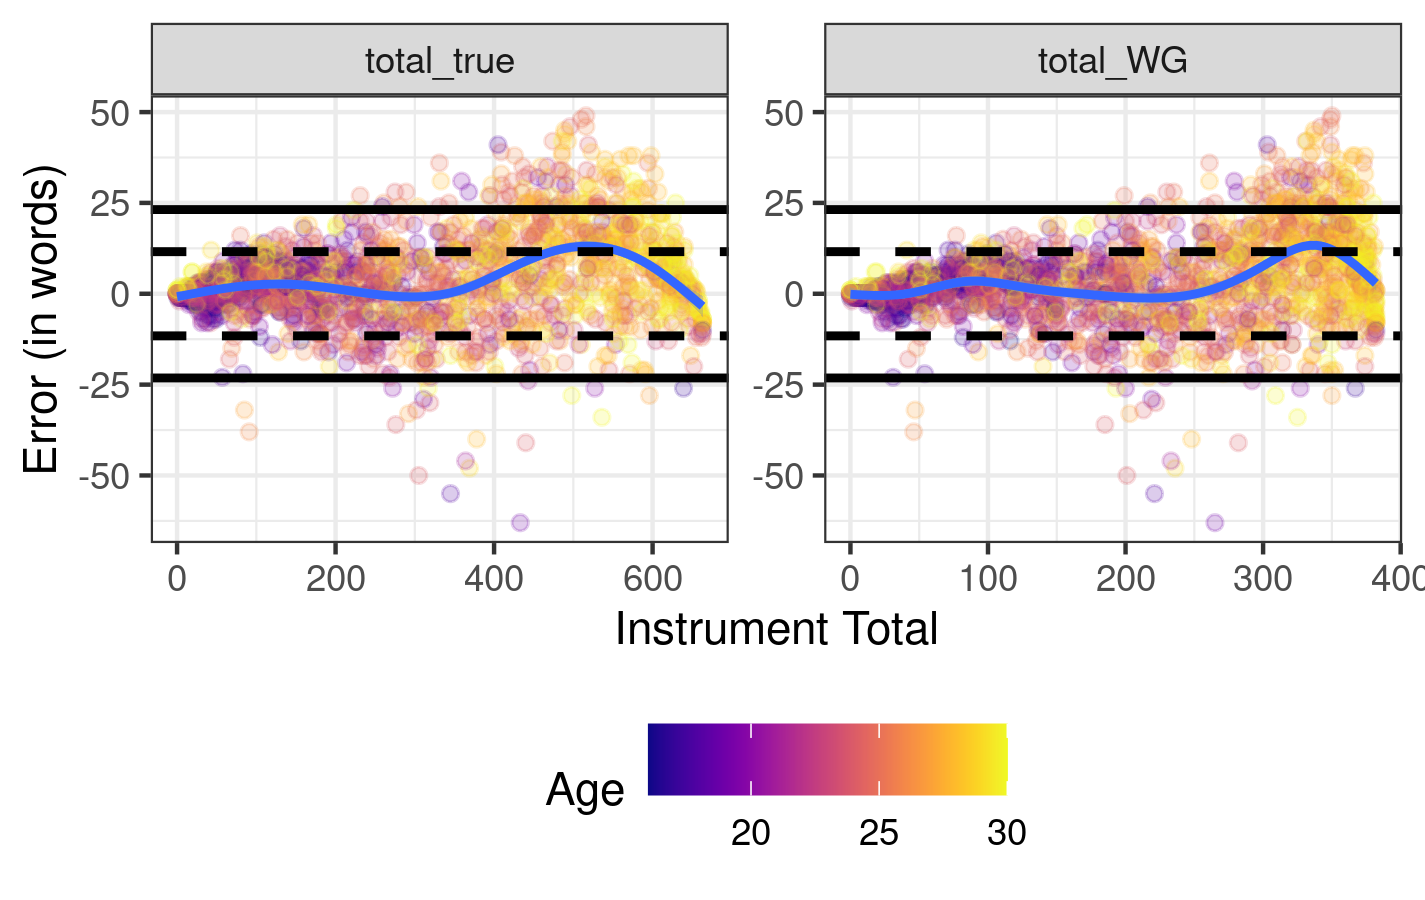
\includegraphics[height=0.3\textheight]{../WG2WS_plots/error_in_words}}

  		\subcaptionbox{Error in percent\label{subfig:errpct}}
    		{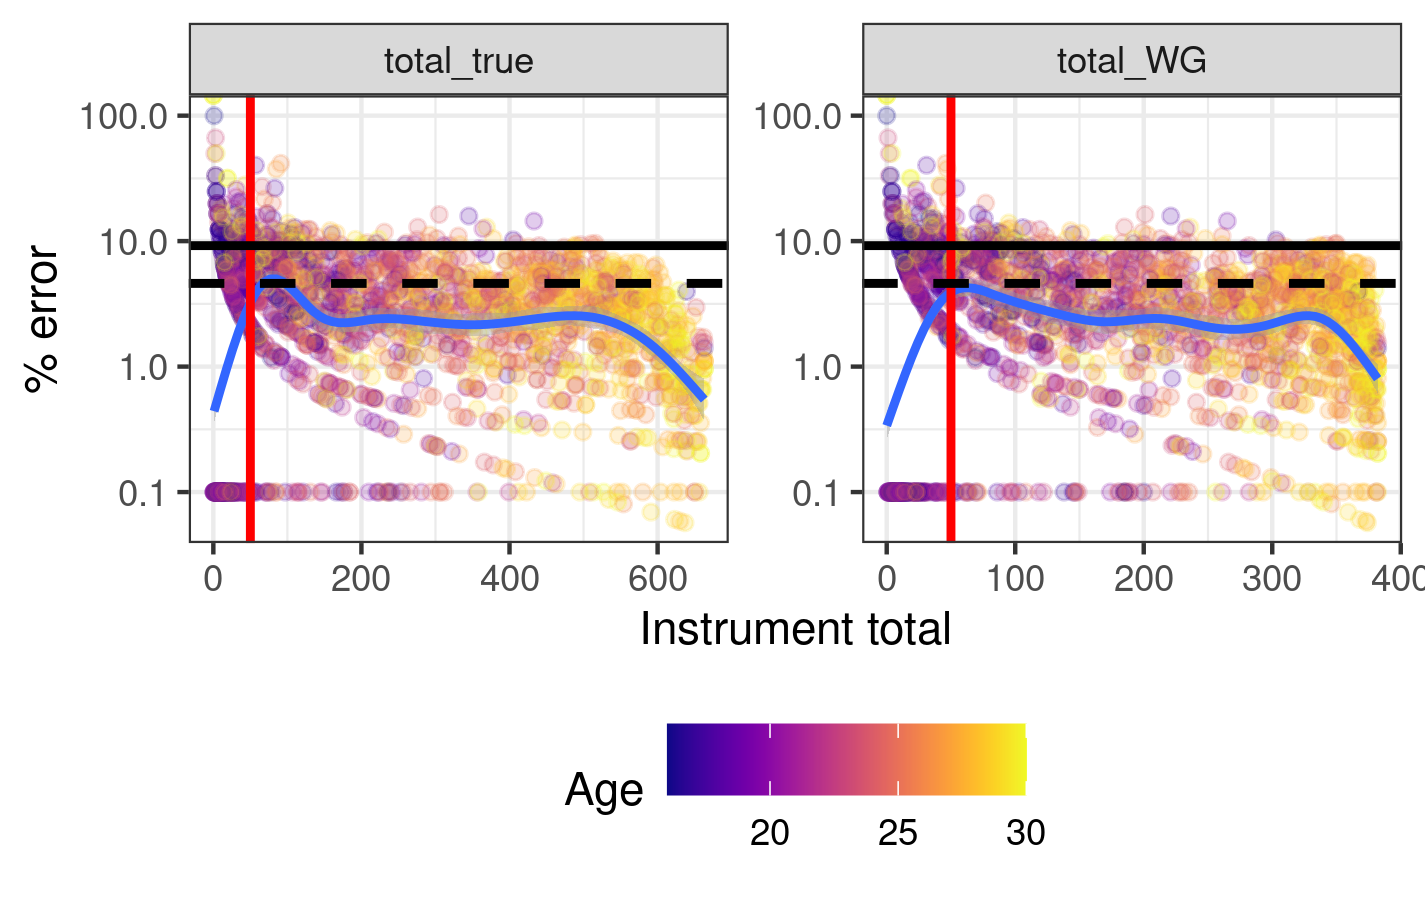
\includegraphics[height=0.3\textheight]{../WG2WS_plots/error_in_pct}}

   		\subcaptionbox{Error in percent by age\label{subfig:errpctage}}
    		{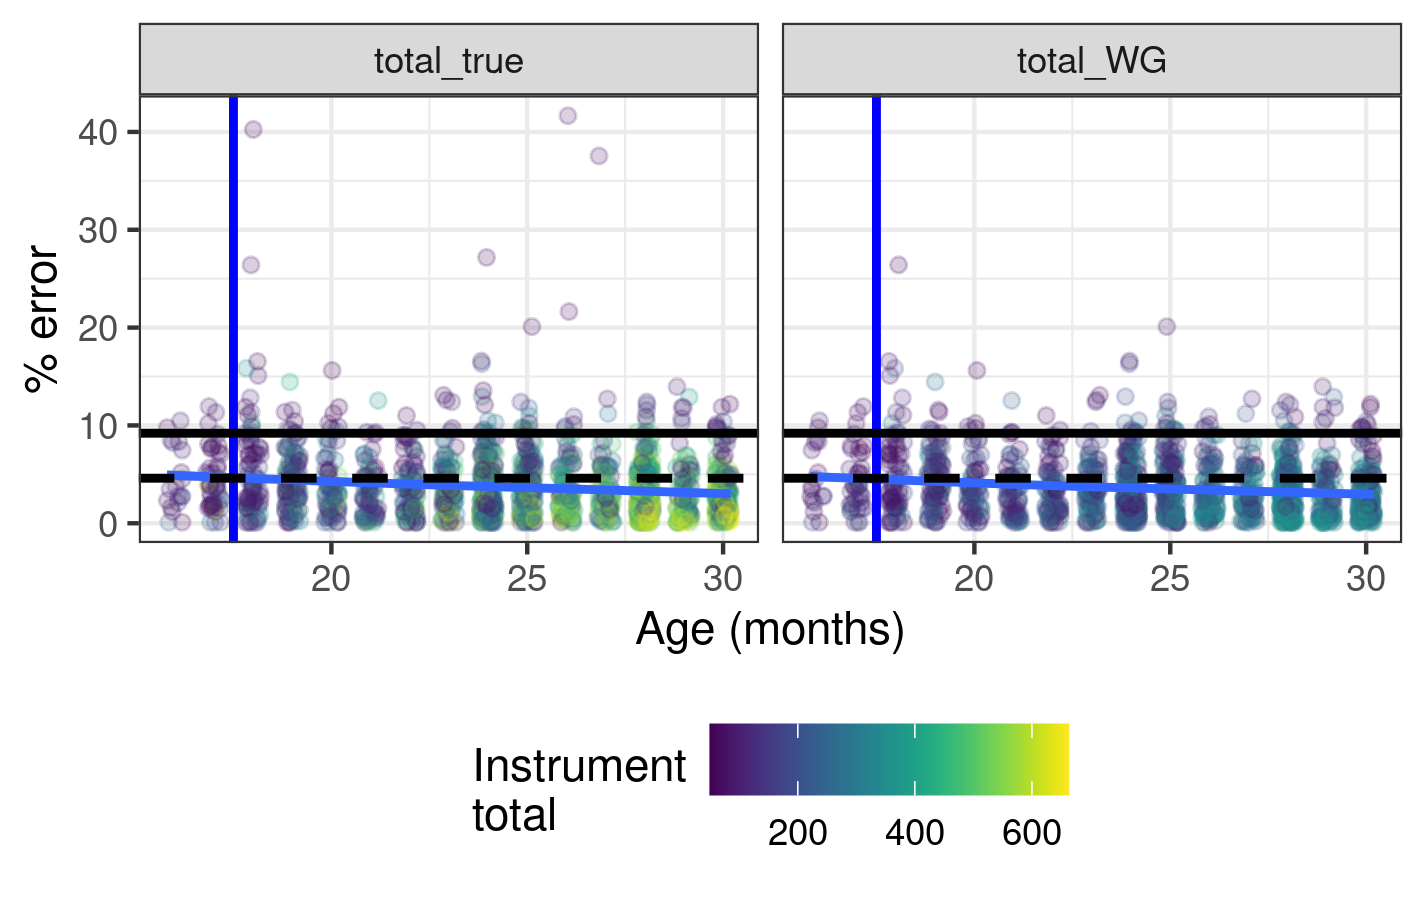
\includegraphics[height=0.3\textheight]{../WG2WS_plots/error_in_pct_by_age}}

    \end{figure}

    \section{Estimating \cwords{}}

    In the training sample, I regressed \cwords{} on age, the quadratic effect
    of age and total \gls{wg} score (and the interaction), and the cubic
    effect of total \gls{wg} score, following the previous analyses. All the
    interaction terms were significant, so all age/total predictors were used
    in the next regression, which included the category score across all other
    categories.

    The second level model offered an improvement in AICc (14802 $\rightarrow$
    13286). For the actual modeling,
    non-significant terms were dropped, leaving:
    WG, WG$^2$, WG$^3$, \textit{Sounds}, \textit{Animals}, \textit{Toys},
    \food, \textit{Clothing}, \textit{Body Parts},
    \textit{Household Items}, \textit{Outside}, \textit{Places},
     \textit{Games \& Routines}, \textit{Action Words},
    \textit{Descriptive Words}, \textit{Question Words}, \textit{Locations},
    age$\times$WG, and
    age$^2\times$WG$^2$
    (where \textit{WG} is the instrument total score).

    Because the number of \cwords{} is low, the variability in predicted score
    was high: error between 0 to 5 words in the test set. Mean \gls{rpd} was
    higher for higher ground-truth \cwords{} scores
    (0: 0.12; 1: 0.27; 2: 0.30; 3: 0.31; 4: 0.31; 5: 0.52; 6: 0.629).
    These are all excellent ``inter-rater reliability'' scores.

    \section{Summary}

    I tested inter-rater reliability using \gls{icc} across three models:
    (1) the base model using the middle 20 categories; (2) adding
    \textit{Sounds}; and (3) adding the \cwords{} estimate. This was done for
    both all participants and those with more than 100 WG words. The \gls{icc}
    for the all-participants models was 0.998 for all input values; and for
    the $\ge100$-participants models was 0.996.

%    (\autoref{table:icc})
%
%    \begin{table}
%
%        \centering
%
%        \caption{\gls{icc} for three models tested on all test participants
%                    and those with more than 100 words only.}
%
%        \label{table:icc}
%
%        \begin{tabular}{crr}
%            \toprule
%            \textbf{Model} & \textbf{ICC\textsubscript{all}} &
%                \textbf{ICC\textsubscript{100w}} \\
%              & $n=1970$ & $n=1294$ \\
%            \midrule
%            1 & 0.998 & 0.996 \\
%            2 & 0.998 & 0.996 \\
%            3 & 0.998 & 0.996 \\
%            \bottomrule
%        \end{tabular}
%
%    \end{table}

    \section{Conclusion}

    \gls{ws} inventory scores can be estimated from \gls{wg} scores with less
    than 15\% mean error using WG total score, inventory score, and age.  For
    very small inventories (less than 50--100), the percent error is elevated,
    however the true error in words remains small. I recommend not using this
    technique on individuals with less than 50 words (or 100 more
    conservatively).

    \cwords{} can be estimated using the rest of the form, however,
    given the low number of items ($n=6$), it may be best to eliminate this
    category from relevant analyses.

\end{document}